\section{Supersafety to Perfect Timeliness}\label{sec:backward-reduction}

We now construct a perfectly timely protocol $\Pi^*$
using a black-box reduction from a supersafe, and live($u$) protocol $\Pi$.
Each honest party $P$, executing the $\Pi^*$ protocol, runs a
full node of protocol $\Pi$.
The ledger of party $P$ for protocol $\Pi$ and $\Pi^*$ is denoted as $\Ledger[][P][r]$ and
$\Ledger[*][P][r]$ respectively.
To construct temporal ledger $\Ledger[*][][r]$,
new transactions appearing in
$\Ledger[][][r]$ are appended to $\Ledger[*][][r - 1]$ with recorded round $r$.
This process is illustrated
in Figure~\ref{fig:backward-reduction}
and the pseudocode is presented in Algorithm~\ref{alg:backward-reduction}.

\begin{figure}
  \centering
  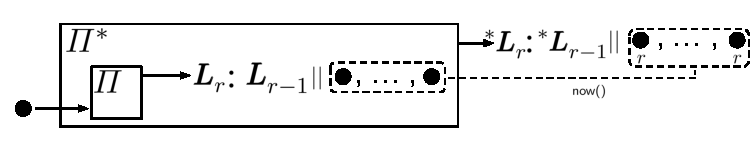
\includegraphics[width=0.9\columnwidth,keepaspectratio]{figures/backward-reduction.pdf}
  \caption{The reduction from Supersafety
    (the $\Pi$ protocol) to Perfect Timeliness (the $\Pi^*$ protocol).
    New transactions of $\Ledger[][][r]$ are included in
    $\Ledger[*][][r]$ with recorded round $r$.
  }
 \label{fig:backward-reduction}
\end{figure}

\import{./}{algorithms/algorithm-backward-reduction.tex}

%We now prove that protocol $\Pi^*$ is perfectly timely.

\begin{theorem}[Supersafety to Perfect Timeliness] \label{thm:backward-reduction}
  An execution of protocol $\Pi^*$ is perfectly timely, supersafe, and live($u$), if the execution of
  protocol $\Pi$ is supersafe and live($u$).
\end{theorem}
\begin{proof}
  Timeliness requirements (1) and (2) are directly satisfied.
  For (3) consider any honest party $P$ and any rounds $r_1 \leq r_2$.
  Only transactions with recorded round greater
  than $r_1$ appear in ledger $\Ledger[*][P][r_2]{[|\Ledger[*][P][r_1]|{:}]}$.
  Hence, $\Pi^*$ is timely with parameter $v = 0$.
  Supersafety and liveness($u$) follow from those of $\Pi$.
  \Qed
\end{proof}
